\documentclass[../main.tex]{subfiles}
\begin{document}
    \chapter{Quantifying allosteric communication via both concerted structural changes and conformational disorder} \label{ch:CARDS}
    

    \graphicspath{{Chapter3/}}
    \captionsetup{labelfont=bf}
    
    \textit{The work in this chapter is published in: Singh, S., 
    and Bowman, G.R., Quantifying allosteric communication via both concerted 
    structural changes and conformational disorder with CARDS. Journal of 
    Chemical Theory and Computation. 13:1507-1517, 2017. PMID: 28282132., Copyright 2018 American Chemical Society} \cite{Singh:2017hh} 
    
    \section{Abstract}
    Allosteric (i.e. long-range) communication within proteins is crucial for many biological processes, such as the activation of signaling cascades in response to specific stimuli. However, the physical basis for this communication remains unclear. Existing computational methods for identifying allostery focus on the role of concerted structural changes, but recent experimental work demonstrates that disorder is also an important factor. Here, we introduce the Correlation of All Rotameric and Dynamical States (CARDS) framework for quantifying correlations between both the structure and disorder of different regions of a protein. To quantify disorder, we draw inspiration from methods for quantifying “dynamic heterogeneity” from chemical physics to classify segments of a dihedral’s time evolution as being in either ordered or disordered regimes. To demonstrate the utility of this approach, we apply CARDS to the Catabolite Activator Protein (CAP), a transcriptional activator that is regulated by Cyclic Adenosine MonoPhosphate (cAMP) binding. We find that CARDS captures allosteric communication between the two cAMP-Binding Domains (CBDs). Importantly, CARDS reveals that this coupling is dominated by disorder-mediated correlations, consistent with NMR experiments that establish allosteric coupling between the CBDs occurs without a concerted structural change. CARDS also recapitulates an enhanced role for disorder in the communication between the DNA-Binding Domains (DBDs) and CBDs in the S62F variant of CAP. Finally, we demonstrate that using CARDS to find communication hotspots identifies regions of CAP that are in allosteric communication without foreknowledge of their identities. Therefore, we expect CARDS to be of great utility for both understanding and predicting allostery. 
        
    \section{Introduction}
    Despite its fundamental importance, understanding of the physical mechanisms of allosteric communication remains incomplete. For example, significant effort has gone into studying how G-Protein Coupled Receptors (GPCRs) allosterically transmit extracellular signals to intracellular binding partners\cite{Rosenbaum:2009id}. However, understanding of this process is still insufficient for the routine design of drugs that allosterically modulate GPCRs\cite{Shoichet:2012fm}.

    Models of allostery have typically focused on concerted structural changes\cite{Guo:2016hv}. For example, the classic induced fit model postulates that ligand binding to one subunit of a protein causes a conformational change in other subunits\cite{Koshland:1959ft,KoshlandJr:1966ffa}. The conformational selection model also focuses on structural changes, positing that ligand binding to one subunit stabilizes an alternative (but pre-existing) structure of other subunits\cite{Monod:1965io}. Extensive work establishes there is often a role for conformational selection\cite{Changeux:2011fv}, though there is clearly a continuum between extreme versions of induced-fit and conformational selection\cite{Csermely:2010cv,Silva:2011ct,Hammes:2009im}. This conclusion implies allostery can be inferred from proteins’ equilibrium fluctuations even in the absence of an allosteric perturbation. Inspired by this implication, numerous methods have been developed to infer allosteric communication from structural fluctuations observed in molecular simulations\cite{Ichiye:1991db,and:1999bo,PratulKAgarwal:2002dp,Agarwal:2002ema,Rod:2003vm,Lange:2006gv,Whitley:2009uq,Weinkam:2012jf,Lenaerts:2008kn,McClendon:2009gd,Dubay:2011ey,Feher:2014cx,Fenwick:2014fc,Cui:2008cc,Elber:2011dj,VanWart:2014dc,Malmstrom:2015kp,Chu:2005gh,Ravindranathan:2005ff,Weinkam:2013fj,Liu:2012em,Zhang2012}.

    While concerted structural changes are clearly important for allostery, there is mounting evidence that conformational disorder has an important role to play, and can even lead to allosteric communication in the absence of concerted structural ,transitions\cite{Guo:2016hv,Kern:2003fv,Tzeng:2011by,Hilser:2007je,Burger:2016gy,Haliloglu:2015dj,HenzlerWildman:2007jb,Hilser:2012em}. The importance of allostery without conformational change first appeared in a model where ligand binding perturbs the entropy of a distant site rather than its preferred structure\cite{Cooper:1984tb}. Since then, NMR and ITC experiments on Catabolite Activator Protein (CAP) have established allosteric communication without conformational change exists in nature\cite{Wand:2013dz,Popovych:2006js,Jakob:2014cp}. CAP is a homodimeric transcription factor whose DNA-binding affinity increases upon binding of cAMP to the cAMP-Binding Domains (CBDs)\cite{Harman:2001td,Heyduk:1989wb}. In wild-type CAP, cAMP binding allosterically induces the DNA-Binding Domains (DBDs) to swivel around the central hinge region into a DNA-binding conformation (Fig. \ref{fig:cap-intro-figure})\cite{Schultz:1991uh,Seok:2014cs}. There is also negative coupling between the two CBDs\cite{Harman:2001td,Heyduk:1989wb,Popovych:2009iu}. A combination of NMR and ITC measurements reveal that binding of cAMP to one CBD reduces the cAMP-binding affinity of the second CBD without changing its structure\cite{Popovych:2006js,Popovych:2009iu}. Additional experiments reveal that binding of cAMP activates the S62F variant of CAP without causing a conformational change in the hinge or DBDs\cite{Tzeng:2009im,Tzeng:2012cu}.


    \begin{figure}[!htb] %Positioning code for figure
        \centering
        \includegraphics[width=4.5in]{cap-intro-fig.eps}
        \caption[Structures of CAP in apo and holo forms.]
            {Structures of CAP in apo and holo forms. \textbf{A.} Structure of apo-CAP, with cAMP-binding domains (CBDs) and DNA-binding domains (DBDs) indicated by brackets. Residues that make up the hinge region are colored in red. \textbf{B.} Structure of holo-CAP with cAMP ligands (spheres) bound to the CBD regions. The same hinge residues are colored in red.}
        \label{fig:cap-intro-figure}
    \end{figure}

    While the importance of disorder is gaining widespread acceptance, the field lacks systematic methods for identifying allosteric communication in the absence of conformational change. For example, NMR has yet to uncover how these signals are transmitted. COREX/BEST\cite{Hilser:2007je,Hilser:1998cj,Hilser:1996ft}, other coarse-grained models\cite{Weinkam:2012jf}, and normal modes\cite{Marcos:2011dr} provide valuable insights but miss essential subtleties, such as important side-chain motions. Using molecular dynamics simulations to measure the mutual information between the orientations of different dihedral angles captures the reduction in uncertainty (measured with an entropy metric) about the structure of one dihedral given knowledge of another\cite{Lenaerts:2008kn,McClendon:2009gd,Dubay:2011ey}, but does not capture phenomena like changes in the rotameric state of one dihedral increasing the conformational heterogeneity of a distant site. Approaches for inferring allosteric coupling from sequence covariation\cite{Lockless:1999uf,Suel:2003ca} are agnostic to the mechanism underlying this communication and cannot explain how it occurs. A method for identifying timing correlations has promise for capturing disorder-mediated coupling\cite{Lin:2016gi}. For example, application of this approach to side-chain degrees of freedom in CAP successfully identified hotspots for allosteric communication.  It also demonstrated that disorder-mediated correlations give rise to long-range communication, while purely structural correlations are limited to short-ranged communication. However, timing correlations do not integrate structural and dynamical correlations into a holistic measure of communication that can capture the continuum of possibilities between purely structural and purely disorder-mediated coupling. 

    Here, we introduce the CARDS (Correlation of all Rotameric and Dynamical States) methodology for quantifying the roles of both concerted structural changes and conformational disorder. CARDS is based on our observation that a single degree of freedom (e.g. a dihedral angle) can transition between “ordered” regimes, wherein it undergoes small fluctuations within a single structural state, and “disordered” regimes wherein it undergoes bursts of transitions between different structural states (Fig. \ref{fig:cards-workflow-fig}). Similar “dynamic heterogeneity”\cite{Ediger:2000ed,Glotzer:2000fy,Richert:2002fa} has been observed in the physics of glasses, where it has been shown that a single degree of freedom’s local environment can either facilitate dynamics by flattening out the effective free energy surface that degree of freedom experiences or freeze out dynamics\cite{Merolle:2005kx,Hedges:2007fw,Keys:2011ut}. CARDS identifies ordered and disordered regimes based on two kinetic signatures: the average time a degree of freedom persists within a structural state and the typical timescale for transitions between structural states. For many dihedrals, we observe that the typical time that elapses between structural transitions, which is dominated by segments of a trajectory in disordered regimes, is orders of magnitude smaller than the typical persistence time in a state. Based on these kinetic signatures, CARDS assigns segments of trajectories to dynamical states (i.e. ordered and disordered regimes). CARDS then quantifies correlations between the structural and dynamical states of different dihedrals. Specifically, we employ the mutual information to assess how much better one can predict the structural and dynamical states of one dihedral given knowledge of the structural and dynamical states of another dihedral. To demonstrate the utility of CARDS, we assess whether it can identify allosteric communication in the absence of concerted structural changes observed in CAP.


    \section{Theory and methods}
    CARDS captures all forms of correlated fluctuations, including concerted structural changes, correlations between the conformational disorder of different degrees of freedom, and correlations between the structure of one degree of freedom and the conformational disorder of another. As in other recent work, we focus on dihedral angles, as they are natural degrees of freedom for describing protein structure and dynamics and are easily decomposed into a small number of rotameric states\cite{McClendon:2009gd,Dubay:2011ey}.

    \begin{figure}[!htb] %Positioning code for figure
        \centering
        \includegraphics[width=5in]{cards-workflow-fig.eps}
        \caption[Workflow for identifying ordered and disordered regimes.]
            {Workflow for identifying ordered and disordered regimes. \textbf{A.} An example of the time-evolution of a $\chi_1$ angle. The core of each rotameric state is shaded green and the buffer zones between them are white. \textbf{B.} Assignment of each snapshot in the trajectory to rotameric states. \textbf{C.} Transition indicator function identifying where the dihedral changes states. Examples of ordered ($\tau_{ord}$) and disordered ($\tau_{dis}$) times are labeled. \textbf{D.} Assignment of each snapshot in the trajectory to dynamical states (e.g. ordered and disordered regimes).}
        \label{fig:cards-workflow-fig}
    \end{figure}
    
    \subsection{Molecular Dynamics simulations}
        We ran three 500 ns simulations with our previously published protocol\cite{Hart:2016kb} (see SI for details). Briefly, we placed PDB ID 4N9H\cite{Seok:2014cs} in a dodecahedron box and solvated it with TIP3P explicit solvent\cite{Jorgensen:1983fl} extending 1 nm beyond the protein in any dimension. We used PyMOL\cite{DeLano:2010wf} to mutate Ser62 to Phe to create a starting structure for the S62F variant.  For each system, we ran simulations with the Gromacs software package\cite{VanDerSpoel:2005hz} using the Amber03 force field\cite{Duan:2003gt}. This combination of software and parameters was selected because it has proven reliable in our past studies of both protein folding\cite{Bowman:2011bc} and structural fluctuations within folded proteins\cite{Hart:2016kb,Bowman:2015dh,Bowman:2015da}.
        As described in the Results section, our microsecond timescale simulations are sufficient to recapitulate much of what is known from experiments about allostery in CAP. The correlation coefficient between the couplings obtained from any individual simulation and the combination of three simulations is 0.64$\pm$0.02, suggesting that hundreds of nanoseconds of simulation may be sufficient to discover gross patterns of communication but are insufficient to obtain converged results.  The correlation coefficient between the coupling obtained from any pair of simulations and the combination of three simulations is 0.79$\pm$0.02, suggesting that 1-1.5 microseconds of simulation give more reproducible results. Taken together with our past work, we conclude that a few microseconds of simulation are adequate to demonstrate the utility of our new method and, likely, to gain valuable insights into many systems.

    \subsection{Assignment of dihedrals to rotameric states}
        Dihedral angles were calculated with MDTraj \cite{McGibbon:2015fv} and assigned to discrete rotameric states (e.g. gauche+, gauche-, and trans for most $\chi$ angles and cis or trans states for backbone dihedrals). Transition-Based Assignment (TBA) is used to distinguish lasting transitions from transient fluctuations\cite{Hummer:2004kb,Bolhuis:2002ew,Buchete:2008hb,Schutte:2011gs}. TBA prevents over-counting of transitions (e.g. due to fluctuations at a barrier peak where a simulation repeatedly crosses a hard cutoff between rotameric states) by defining a core region within each rotameric state and buffer zones between them. A dihedral is only considered to have changed rotameric states if it transitions from the core of one state to the core of another state, passing completely through the buffer zone between cores (Fig. \ref{fig:cards-workflow-fig}A and \ref{fig:cards-workflow-fig}B). A dihedral that starts in one core, enters a buffer zone, and then returns to its initial core is said to have remained in the initial rotameric state. We define the core of a rotameric state as a region of width W centered between the boundaries between rotamers. We present results using a core width of 90°, but our results are robust to variations in the core width ranging from 60° to 90° (Fig. \ref{fig:cards-pearsonr-fig}A)

    \subsection{Assignment of snapshots to dynamical states}
        CARDS assigns snapshots to ordered and disordered regimes based on two variables that describe the dynamics of the trajectory: the mean ordered time ($\tau_{ord}$) and mean disordered time ($\tau_{dis}$). An ordered time ($\tau_{ord}$) is the time from any time-point to the next time where a transition occurs and a disordered time ($\tau_{dis}$) is the time between two consecutive transitions (Fig. \ref{fig:cards-workflow-fig}C). These times are called persistence and exchange times in the condensed matter physics literature\cite{Hedges:2007fw,Keys:2011ut,Jung:2005jk}. For many dihedrals, we observe that $\langle\tau_{dis}\rangle \ll \langle\tau_{ord}\rangle$ because (〈$\tau_{dis}$〉) is dominated by the short times between transitions in disordered regimes, whereas 〈$\tau_{ord}$〉 is heavily influenced by the lengthy times without any transitions in ordered regimes. To calculate these times, CARDS first identifies the time points where a dihedral transitions between two different rotameric states (Fig. \ref{fig:cards-workflow-fig}C), referred to as the transition indicator function. The method then extract the complete set of $\tau_{dis}$ and $\tau_{ord}$ values in the trajectory. Next, CARDS classifies each segment of a trajectory between two consecutive transitions as being in an ordered or disordered regime based on whether the length of the segment $t$ between the transitions is more consistent with the distribution of ordered or disordered times (Fig. \ref{fig:cards-workflow-fig}D). We find that transitions within ordered and disordered regimes are roughly Poisson processes with different characteristic times ($\langle\tau_{ord}\rangle$ and〈$\tau_{dis}$〉, respectively), see Fig. \ref{fig:cards-timescale-dists-fig}. Therefore, CARDS determines if a segment of a trajectory of length $t$ between two consecutive transitions is more consistent with an ordered or disordered regime using the likelihood ratio ($L$):
        \begin{equation}\label{likelihood-ratio-eq}
        L(t)=\frac{P_{dis}(t)}{P_{ord}(t)}=\frac{(\frac{1}{\langle\tau_{dis}\rangle})e^{-\frac{t}{\langle\tau_{dis}\rangle}}}{(\frac{1}{\langle\tau_{ord}\rangle})e^{-\frac{t}{\langle\tau_{ord}\rangle}}}
        \end{equation}
        where $P_{dis}$ is the probability the segment is disordered and $P_{ord}$ is the probability it is ordered. Taking inspiration from the interpretation of Bayes factors\cite{Kass:2012bb}, CARDS classifies a segment of a trajectory as being disordered if $L>3.0$, otherwise the trajectory segment is classified as being in an ordered regime. Our results are robust to varying this cutoff from 1.5 to 5 (Fig. \ref{fig:cards-pearsonr-fig}B).

    \subsection{Calculation of structural, disorder-mediated, and holistic correlations}
        The primary objective of CARDS is to calculate the total correlation between different dihedrals, including both their rotameric state and dynamical state (e.g. whether the dihedral is in an ordered or disordered regime at a given time). Towards this end, we define the holistic correlation ($I_H$) between dihedrals $X$ and $Y$ as
        \begin{equation}\label{holistic-mut-inf-eq}
            % \binom{n}{k} = \frac{n!}{k!(n-k)!}
            I_{H}(X,Y) = \overline{I_{ss}(X,Y)}+\overline{I_{dd}(X,Y)}+\overline{I_{ds}(X,Y)}+\overline{I_{sd}(X,Y)}
        \end{equation}
        where $\overline{I_{ss}(X,Y)}$ is the normalized mutual information between the structure (i.e. rotameric state) of dihedral $X$ and the structure of dihedral $Y$, $\overline{I_{sd}(X,Y)}$ is the normalized mutual information between the structure of dihedral $X$ and the dynamical state of dihedral $Y$, $\overline{I_{ds}(X,Y)}$ is the normalized mutual information between the dynamical state of dihedral X and the structure of dihedral Y, and $\overline{I_{dd}(X,Y)}$ is the normalized mutual information between the dynamical state of dihedral $X$ and the dynamical state of dihedral $Y$. The mutual information (I) is:
        \begin{equation}\label{mut-inf-eq}
            I(X,Y) = -\sum_{x \in X}\sum_{y \in Y} {{\frac{P(x,y)}{P(x)P(y)}}}
        \end{equation}
        where $x \in X$ refers to the set of possible states that dihedral $X$ can adopt, $p(x)$ is the probability that dihedral $X$ adopts state $x$, and $p(x,y)$ is the joint probability that dihedral $X$ adopts state $x$ and dihedral $Y$ adopts state $y$. We define the normalized mutual information ($\overline{I(X,Y)}{}$) as 
        \begin{equation}\label{normalized-mi-=eq}
            \overline{I(X,Y)}=\frac{I(X,Y)}{C(X,Y)}
        \end{equation}
        where $C(X,Y)$ is the maximum possible mutual information between two dihedrals, called the channel capacity\cite{witten2002data}. Using this normalized mutual information allows for a direct comparison between the different components of the holistic correlation by correcting for the fact that the largest possible mutual information between different types of dihedrals will vary based on how many different states there are. For example, a side-chain dihedral has three possible rotameric states but only two possible dynamical states, so structural correlations ($I_{ss}$) can be as large as $log(3)$ while the correlations between dynamical states ($I_{dd}$) can only reach as high as $log(2)$. 

        In addition to the above, we define the disorder-mediated correlation ($I_{DM}$) as all forms of correlation between two dihedrals that rely, at least in part, on disorder ($\overline{I_{sd}}+\overline{I_{ds}}+\overline{I_{dd}}$). This construct is useful for assessing the importance of disorder relative to existing methods based purely on concerted structural changes ($I_{ss}$). We use bootstrapping to measure the uncertainty in our estimates of all the components of the holistic correlation to ensure any comparisons we make are statistically sound. Specifically, we draw 20 random samples of our trajectories, with replacement, and calculate the structur{}al and disorder-mediated correlations between all pairs of residues. We conclude that disorder-mediated communication dominates if the average disorder-mediated communication minus the standard deviation across all our bootstrap samples is greater than the mean structural correlation plus the standard deviation.

    \subsection{Calculation of net communication to a target site}
        We are often interested in calculating how much influence a particular residue has over another site, such as an active site or ligand-binding site. To calculate the communication between a reference residue and some target site, we take the average mutual information between two sets of dihedrals: 1) all dihedrals in the reference residue and its nearest neighbors and 2) all dihedrals in the target site. We define the nearest neighbors of a reference residue as all residues with atoms that fall within 3 \AA{} of any atom in the reference residue. Varying this cutoff does not alter our results (Fig. \ref{fig:cards-pearsonr-fig}C). Including both a reference residue and its nearest neighbors accounts for the fact that mutating the reference residue will directly change the environment of all neighboring residues.

    \subsection{Calculation of global communication}
        In addition to identifying residues that have strong correlations to a specific target site, it would also be valuable to identify residues that generally appear to play an important role in allosteric networks. Towards this end, we define the global communication strength of a residue as the sum of its holistic correlations to all other residues. For these calculations, we also include neighboring residues, as in our calculation of the net communication to a target site.

    \section{Results and discussion}
    \subsection{Many dihedrals have the potential for disorder-mediated communication}
        For a dihedral to have ordered and disordered regimes, 〈$\tau_{ord}$〉 must be significantly larger than 〈$\tau_{dis}$〉. We reasoned that determining if ${\langle\tau_{ord}\rangle} \geq { 3\times\langle\tau_{dis}}\rangle$  is a reasonable heuristic for identifying dihedrals with separable ordered and disordered regimes based on the likelihood ratio defined in Eq. \ref{likelihood-ratio-eq}. Dihedrals that do not meet this criterion are classified as entirely being in ordered regimes and, therefore, are only capable of having structural correlations with other dihedrals. 

        Based on the criterion defined above, we find that 556 of the 1584 dihedrals in CAP have separable ordered and disordered regimes and, therefore, are capable of disorder-mediated communication with other dihedrals (Fig. \ref{fig:cards-avgtimes-2dhist-fig}). Mapping these dihedrals to the apo structure of CAP highlights a number of interesting patterns (Fig. \ref{fig:cap-disordered-resis-fig}). First of all, CARDS reveals that many side-chain dihedrals buried in CAP’s core are capable of disorder-mediated communication. This finding helps to rectify the apparent contradiction between the common physical intuition that proteins’ cores should be rigid due to their tight packing and the observation that there is substantial conformational heterogeneity within proteins’ cores\cite{Fraser:2011jf,bowman2014extensive}. That is, dihedrals within a protein’s core are commonly locked in a single rotameric state for extended periods of time but rare fluctuations create room for conformational changes. Backbone dihedrals that are capable of disorder-mediated communication tend to reside on the protein’s surface. Notably, a number of these backbone dihedrals are in $\beta$-sheets that contact cAMP. However, there are also backbone dihedrals within the core that are capable of disorder-mediated communication. For example, we find backbone dihedrals within the central hinge region that are capable of disorder-mediated communication. This observation is noteworthy because the hinge region undergoes a large conformational change upon activation of CAP (Fig. \ref{fig:cap-intro-figure})\cite{Popovych:2009iu,Tzeng:2009im,Tzeng:2012cu}. We find that similar patterns emerge when we vary the cutoff for determining whether a dihedral has separable ordered and disordered regimes (Fig. \ref{fig:cards-disord-resis-cutoff}). In the future it will be interesting to examine whether separate proteins, or homologous members of a family, have similar proportions and patterns of dihedrals that are separable into ordered and disordered regimes. However, given the opportunity to only analyze a limited number of sufficiently sampled datasets so far\cite{Cruz2020vp35m,Sun:2018kx,porter_conformational_2020}.

    \begin{figure}[!htb] %Positioning code for figure
        \centering
        \includegraphics[width=4.5in]{cap-disordered-residues-fig.eps}
        \caption[Residues whose dihedrals are capable of disorder-mediated communication.]
            {Residues whose dihedrals are capable of disorder-mediated communication. \textbf{A.} Residues with at least one backbone dihedral that is capable of disorder-mediated communication (orange). \textbf{B.} Residues with at least one side-chain dihedral that is capable of disorder-mediated communication (green).}
        \label{fig:cap-disordered-resis-fig}
    \end{figure}

    \subsection{Disorder-mediated correlations dominate communication between the CBDs}
        Given experimental evidence for allosteric communication between the CBDs without a concerted structural change\cite{Tzeng:2009im}, we expect the disorder-mediated component of the holistic correlation between these sites to be larger than the purely structural component. To test this prediction, we simulated apo CAP for 1.5 $\mu$s and calculated the net communication of every residue to one of the cAMP-binding sites. Specifically, we defined the target site as all residues with heavy atoms within 6\AA of one of the two cAMP molecules in the holo crystal structure (PDB ID 1CGP)\cite{Schultz:1991uh}. The residues in this target site are 30, 36, 49, 61-62, 64, 69-86, and 99 from chain A and residues 122-129 from chain B.

        As predicted, CARDS successfully identifies that there is communication between the two CBDs. Fig. \ref{fig:cap-targetsite-fig}A shows the holistic correlations to a single cAMP-binding site. Unsurprisingly, the residues with the strongest correlations to this set of residues reside within the same CBD. However, there is also strong communication between the target site and residues lining the other cAMP-binding pocket. There are also strong correlations on the central hinge region and the interface between the CBDs and DBDs that may be responsible for allosteric coupling between these domains.

        To determine the relative importance of disorder-mediated communication and purely structural correlations, we broke the holistic communication into structural and disorder-mediated components. Furthermore, we used bootstrapping to estimate the uncertainty in each of these components.

    \begin{figure}[!htb] %Positioning code for figure
        \centering
        \includegraphics[width=4.5in]{cap-targetsite-fig.eps}
        \caption[Communication to a single CBD.]
            {Communication to a single CBD. \textbf{A.} Holistic mutual information ($I_H$) of each residue to the residues lining a single cAMP-binding pocket (shown in sticks). \textbf{B.} Residues whose communication to the cAMP-binding pocket is dominated by disorder-mediated communication (orange sticks).  Residues lining the target cAMP-binding pocket are in blue sticks.}
        \label{fig:cap-targetsite-fig}
    \end{figure} 

        Identifying residues where disorder-mediated communication to the target cAMP-binding site is larger than purely structural correlations automatically identifies a number of residues in the second cAMP-binding site (Fig. \ref{fig:cap-targetsite-fig}B, Fig. \ref{fig:cards-top5percentresis}). This finding demonstrates that CARDS recapitulates the experimental finding that communication betwen the two CBDs does not primarily occur through concerted structural changes\cite{Tzeng:2009im}. CARDS also identifies disorder-dominated communication within a single CBD. Furthermore, the Pearson correlation coefficient between structural and disorder-mediated communication is 0.44. This result indicates there are some similarities between patterns of allosteric coupling that could be observed by focusing entirely on structural correlations and those identified by CARDS, but that considering disorder provides additional information.

    \subsection{Disorder-mediated communication is enhanced in the S62F variant}
        The S62F variant of CAP is still activated by cAMP binding\cite{Tzeng:2009im,Tzeng:2012cu,Dai:2004ea,Aiba:1985ui}. However, NMR studies have revealed that the conformation of the DBDs does not change upon cAMP binding. Rather, NMR and ITC experiments suggest an important role for conformational entropy, with the DBDs only changing conformation in the presence of both cAMP and DNA\cite{Tzeng:2009im,Tzeng:2012cu}. Therefore, we expect an increase in disorder-mediated communication between the CBDs and DBDs in the S62F variant, compared to wild-type CAP.

        To determine the effect of the S62F variant, we also ran 1.5 $\mu$s of simulation of this variant. Then we calculated the holistic communication to a single cAMP-binding site, as described for wild-type CAP.

        As expected, we observe significant increases in disorder-mediated communication between the target CBD and the DBDs.  There are particularly large increases in disorder-mediated correlations in regions of known importance for CAP activation, such as the central hinge region and along the interfaces between the CBDs and DBDs (Fig. \ref{fig:cap-s62f-deltaMI-fig}A). At the same time, there are some decreases in disorder-mediated communication within the CBDs. There are also changes in purely structural correlations. These changes often follow the same qualitative trends as the changes in disorder-mediated communication. However, the magnitudes of any increases in purely structural correlations are considerably smaller than the increases in disorder-mediated correlations. Furthermore, reductions in structural correlations are often larger than any decreases in disorder-mediated communication.

    \begin{figure}[!htb] %Positioning code for figure
        \centering
        \includegraphics[width=5in]{cap-s62f-deltaMI-fig.eps}
        \caption[Change in coupling to a single CBD pocket upon the S62F mutation.]
            {Change in coupling to a single CBD pocket upon the S62F mutation. \textbf{A.} Change in disorder-mediated communication of each residue to the single cAMP-binding pocket depicted in Fig. \ref{fig:cap-targetsite-fig}. \textbf{B.} Change in structural communication of each residue to the same cAMP-binding pocket. Red indicates increased communication in S62F compared to wild-type, and blue indicates decreased communication.}
        \label{fig:cap-s62f-deltaMI-fig}
    \end{figure} 

    \subsection{Side-chain-side-chain and backbone-side-chain correlations dominate allosteric communication in CAP}
        To begin understanding the relative importance of different types of degrees of freedom, we plotted the matrix of correlations between every pair of dihedrals (Fig. \ref{fig:cap-bb-sc-matrix-fig}A). The upper triangle represents purely structural correlations, while the lower triangle represents purely disorder-mediated correlations. Side-chain and backbone dihedrals are also grouped together to enable comparisons between the relative strengths of backbone-backbone, backbone-side-chain and side-chain-side-chain correlations.
        Inspection of the matrix of all pairwise correlations immediately reveals that side-chain-side-chain correlations dominate allosteric communication in CAP. This observation is consistent with previous reports that side-chain degrees of freedom are more variable than the backbone\cite{Fraser:2011jf,bowman2014extensive,Kurplus:1983ts,brooks2006advances,Depristo:2004tb,Wand:1996hr,LindorffLarsen:2005bi,Igumenova:2006hw,Dubay:2009gv}. Backbone-backbone correlations are far rarer, and we find that disorder-mediated correlations between backbone dihedrals are more common than structural correlations.
        We also find a small number of backbone dihedrals that appear to be hubs of communication that are coupled to the side-chains of a large fraction of the residues in CAP. These hubs appear as lines in the backbone-side-chain quadrants of the matrix in Fig. \ref{fig:cap-bb-sc-matrix-fig}A. Mapping the strongest (top 5\%) backbone hubs to the structure reveals that they cluster in two regions: the phosphate-binding cassette (PBC) of each CBD and the interface between the CBDs and DBDs, including the central hinge (Fig. \ref{fig:cap-bb-sc-matrix-fig}B). Using an even stricter cutoff (top 2\%) only identifies residues along the CBD-DBD interface and within the central hinge (Fig. \ref{fig:cards-top2percenthubs}), further emphasizing their importance in the allosteric network. This result suggests that perturbations to these functionally important regions (e.g. cAMP binding) can influence the behavior of the entire protein, and vice versa.

        It is also possible that the assumed Poissonian distribution of dihedral timescales may impact the degree of measured communication. While these are long-tailed distributions, it is not clear if they are truly Poissonian, and proving this behavior may prove a non-trivial task. While we already observe that our measurements are robust to the choice of Likelihood Ratio cutoff (Figure \ref{fig:cards-pearsonr-fig}). It will be worth exploring whether or not other exponential distributions can be used to more appropriately model the probability of being ordered or disordered when computing a likelihood ratio.

        More importantly, using a different binning strategy than 3-state or 2-state designations can improve measurements of allosteric coupling. These rotameric state designations are based on classic alkane stereochemistry, and assume flat prior. Given the chemical diversity of amino acids, it is possible that some dihedrals will never explore all rotameric states. For example a phenylalanine $\chi _{2}$ will not explore all three possible rotameric states due to the aromatic ring on the sidechain. One possible avenue to improve the measurement of dihedral communication is to incorporate established rotamer libraries into the rotameric state decomposition\cite{chaudhury_pyrosetta:_2010, shapovalov_smoothed_2011}. Using library-based designations,and their standard error measurements to define buffer region widths, would correct the currently-used flat prior. This would increase the reliability of measurement of dihedral communication while still allowing us to assess the role of side-chain dihedrals against backbone dihedrals in communication. However, it is important to note that the current binning strategy being used is robust when assessed with metrics such as bootstrapping or Excess Mutual Information. Excess Mutual Information has been shown as a robust way of detecting noise in measuring allosteric communication, and major dihedral communication patterns are still evident after this correction\cite{Bowman:2012jd}. Consistently, we observe that communication measurements remain significant (ie. not within error of zero) (see Appendix \ref{ch:cards-supp-info} and Figure \ref{fig:cards-pearsonr-fig}). It is worth noting that utilizing this naïve, residue-independent binning system is already capable of making measurable predictions of protein allostery\cite{Sun:2018kx,Cruz2020vp35}.

    \begin{figure}[!htb] %Positioning code for figure
        \centering
        \includegraphics[width=6in]{cap-bb-sc-matrix-fig.eps}
        \caption[Hubs of backbone-side-chain communication in wild-type CAP.]
            {Hubs of backbone-side-chain communication in wild-type CAP. \textbf{A.} Mutual information between every pair of dihedrals in wild-type CAP. The upper triangle of the matrix (above the green diagonal) represents structural communication and the lower triangle (below the green diagonal) represents disorder-mediated communication. The pink and cyan squares encompass the regions of the matrix that capture backbone-side-chain communication that is mediated by disorder-mediated and structural coupling, respectively. \textbf{B.} Structure of wild type CAP highlighting the residues that are the strongest hubs (top 5\%) of backbone-side-chain communication (red sticks).}
        \label{fig:cap-bb-sc-matrix-fig}
    \end{figure} 

    \subsection{Locating communication hotspots identifies key functional sites}
        The coincidence of backbone dihedrals that are hubs of communication and key functional sites suggests that CARDS may be capable of predicting the locations of such sites. Indeed, if evolution has selected for communication between particular sites, then one might expect residues in these sites to have stronger coupling to other regions of a protein than typical residues.
        
        To detect strongly communicating residues, we ranked each residue based on the sum of its correlations to all other residues in the protein. This measure of global communication will highlight two types of hotspots: 1) hubs with correlations to many residues and 2) residues that have strong correlations to a few residues.

        Coloring each residue in the $apo$ structure according to its global communication highlights that the central hinge region and the helices between the two cAMP-binding sites are key mediators of allosteric communication in CAP (Fig. \ref{fig:cap-global-mi-fig}). There are also hotspot residues in other parts of the cAMP-binding sites and along the interfaces between the CBDs and DBDs. These are precisely the regions that were identified by assessing communication to a single cAMP-binding site, providing evidence that CARDS can indeed identify key functional sites without foreknowledge of their locations. This conclusion is further supported by the fact that the central hinge region has even stronger communication in the S62F variant (Fig. \ref{fig:cap-deltaglobalMI}).

    \begin{figure}[!htb] %Positioning code for figure
        \centering
        \includegraphics[width=3.16in]{cap-global-mi-fig.eps}
        \caption[Global communication strength of each residue in apo CAP.]{Global communication strength of each residue in apo CAP.}
        \label{fig:cap-global-mi-fig}
    \end{figure} 

    \section{Conclusion}
        CARDS provides a means to integrate concerted structural changes and disorder-mediated correlations into a holistic view of allostery. Application of this approach to wild-type CAP and the S62F variant demonstrates the method’s ability to identify allosteric coupling in the absence of concerted structural changes. Specifically, we showed that examining the coupling of every residue to a known cAMP binding site naturally highlights regions of the protein that are known to be impacted by cAMP binding, such as the second cAMP binding site and the central hinge region connecting the CBDs and DBDs. Decomposing the correlations between these sites into disorder-mediated and purely structural components demonstrates an important role for disorder-mediated coupling in the absence of concerted structural changes. Our global communication metric also provides a means to identify important functional sites without foreknowledge of their existence and locations. For example, this metric identifies the central hinge region—which undergoes the largest conformational change upon activation—and the cAMP binding pockets as important components of the allosteric network in CAP. Therefore, CARDS should be a powerful means to identify allosteric networks in systems that have not been studied as thoroughly as CAP. Taken together, we expect CARDS to be of great utility for understanding allostery in systems where it is already known to occur, as well as for predicting allostery in systems where it has yet to be observed.

    \section{Acknowledgements}
        This work was funded by NSF CAREER Award MCB-1552471. G.R.B. holds a Career Award at the Scientific Interface from the Burroughs Wellcome Fund and a Packard Fellowship for Science and Engineering from The David $\&$ Lucile Packard Foundation. We are also grateful to NVIDIA Corporation for the GTX Titan X used to run preliminary simulations. Finally, thanks to Kelsey C. Schuster and David Chandler, who, in collaboration with G.R.B., first demonstrated that proteins’ side-chains have dynamic heterogeneity.

    
    % \section{Supplemental Material}
    %     \renewcommand{\thefigure}{\arabic{chapter}.S\arabic{figure}}
    %     \setcounter{figure}{0}
    %     \renewcommand{\theequation}{S\arabic{equation}}
    %     \setcounter{equation}{0}
    % \subsection{Molecular dynamics simulations}
    %     All simulations were carried out on GROMACS (version 5.1.1)\cite{Abraham:2015gj,VanDerSpoel:2005hz} using periodic boundary conditions in a dodecahedron with explicit water solvent. Simulations were carried out at 300K using the AMBER03\cite{Duan:2003gt} force field with the TIP3P water model\cite{Jorgensen:1983fl}. The starting conformations of wild-type apo and cAMP-bound CAP were generated by placing crystallographic structures (PDB ID: 4N9H and 1CGP respectively)\cite{Seok:2014cs,Schultz:1991uh} into separate dodecahedron boxes that extended 1.0 nm from the protein surface in any direction. Starting conformations fore the S62F variant were generated using the PyMol\cite{DeLano:2010wf} mutagenesis tool. Each system was then minimized independently with the steepest-descent algorithm until the maximum force fell below 1000 kJ/mol/min using a step size of 0.01nm and a cutoff distance of 1.2nm for the neighbor list, Coulomb interactions, and van der Waals interactions. For equilibration runs, all bonds were constrained with the LINCS algorithm\cite{Hess:2008fl} and virtual sites\cite{Feenstra:1999ue} were used to allow for a 4fs time step. As before, cut-offs of 1.0 nm were used for the neighbor list, Coulomb interactions, and van der Waals interactions. The Verlet cutoff scheme was used for the neighbor list, and Particle Mesh Ewald\cite{Essmann:1995gi} was employed for the electrostatics (with a grid spacing of 0.12nm, PME order 4, and tolerance 1e-5). The stochastic velocity rescaling (v-scale) thermostat\cite{Bussi:2007cs} was used to hold the temperature at 300K, and the Berendsen barostat\cite{Berendsen:1984fm} was used to bring the system to 1 bar pressure. For the production runs, the position restraint was removed and the Parrinello-Rahman barostat\cite{Parrinello:1981it} was employed. Conformations were stored every 10 ps. For each system, three 500ns runs were conducted totaling to 1.5$\mu$s of aggregate simulation time per system. 

    %     Dihedral angles were extracted using the MDTraj Library\cite{McGibbon:2015fv} (v. 1.7). Mappings were all drawn in PyMol (version 1.7)\cite{DeLano:2010wf}, and all figures were constructed in Inkscape (v. 0.48). 

    % \subsection{Sensitivity analysis}
    %     We varied all the cutoff values employed in the CARDS algorithm to ensure the robustness of our results. Specifically, we varied the core width from 60° to 90°, the likelihood ratio cutoff from 1.5 to 5.0, and the neighbor distance cutoff from 2-6\AA. Fig. \ref{fig:cards-pearsonr-fig} demonstrates that the communication to the CBD does not change dramatically as these parameters are varied.

    % \begin{figure}[!htb] %Positioning code for figure
    %     \centering
    %     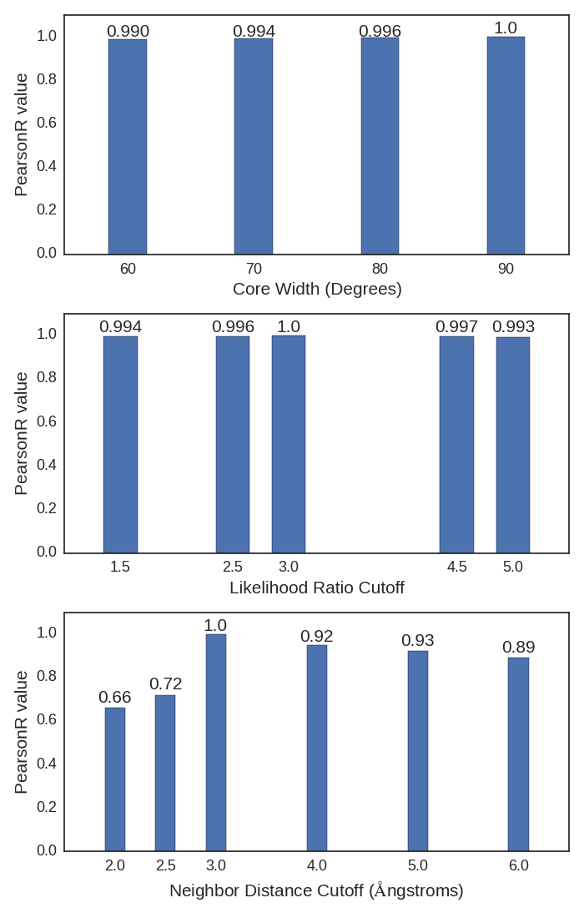
\includegraphics[width=4in]{suppfig1-pearsonr.png}
    %     \caption[]{Pearson Correlation Coefficients (PearsonR) between the CARDS results presented in the main text and those with varying A. the core width, B. the likelihood ratio cutoff, and C. the neighbor distance cutoff.}
    %     \label{fig:cards-pearsonr-fig}
    % \end{figure} 

    % \begin{figure}[!htb] %Positioning code for figure
    %     \centering
    %     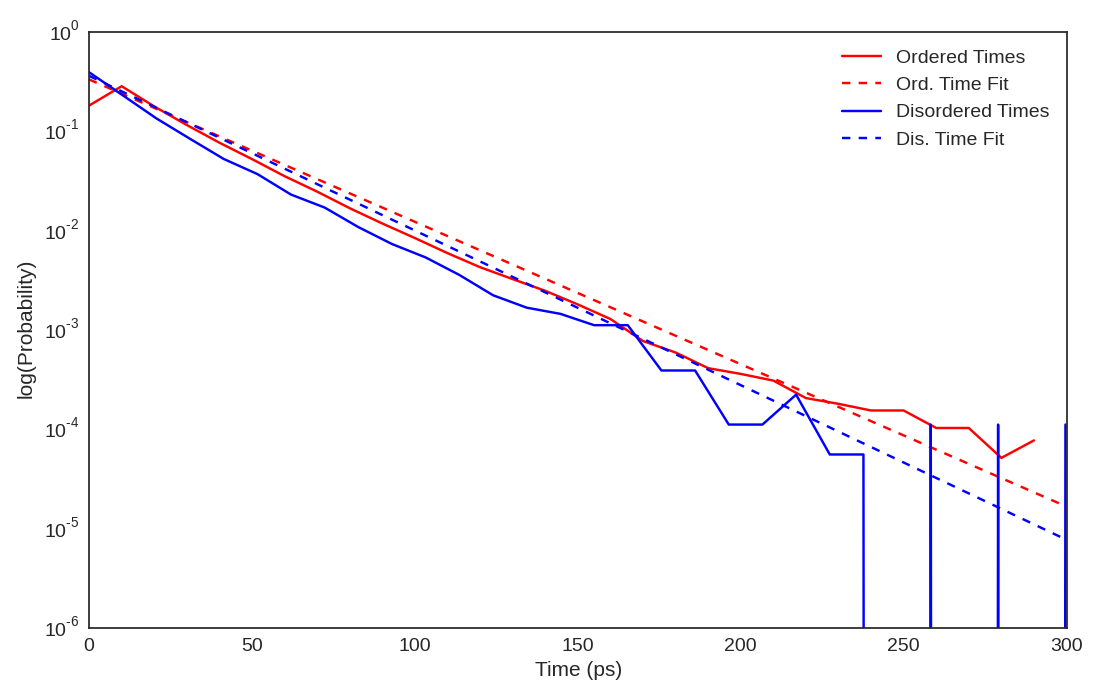
\includegraphics[width=4.5in]{suppfig2-timescale-dists.png}
    %     \caption[]{The distribution of ordered and disordered times for a single dihedral across a single simulation trajectory. The solid lines represent the histogram of times extracted from the trajectory, while the dashed lines represent fits based on the average ordered ($\langle\tau_{ord}\rangle$) and disordered times ($\langle\tau_{dis}\rangle$).}
    %     \label{fig:cards-timescale-dists-fig}
    % \end{figure} 

    % \begin{figure}[!htb] %Positioning code for figure
    %     \centering
    %     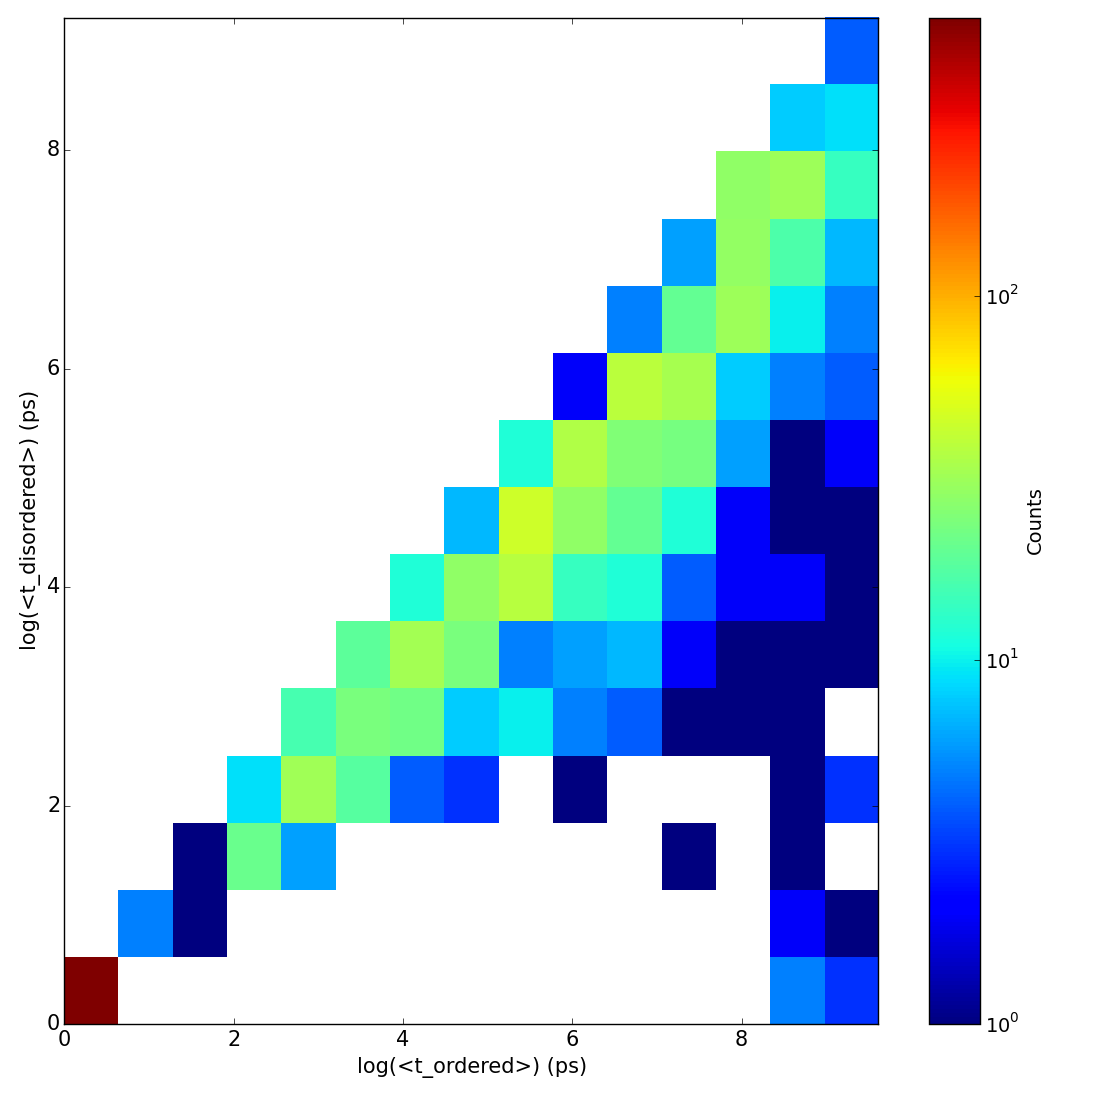
\includegraphics[width=4.5in]{suppfig3-avgtimes-2dhist.png}
    %     \caption[]{Two-dimensional histogram of the average ordered and disordered times ($\langle\tau_{ord}\rangle$ and $\langle\tau_{dis}\rangle$) for all dihedrals in CAP.}
    %     \label{fig:cards-avgtimes-2dhist-fig}
    % \end{figure} 

    % \begin{figure}[!htb] %Positioning code for figure
    %     \centering
    %     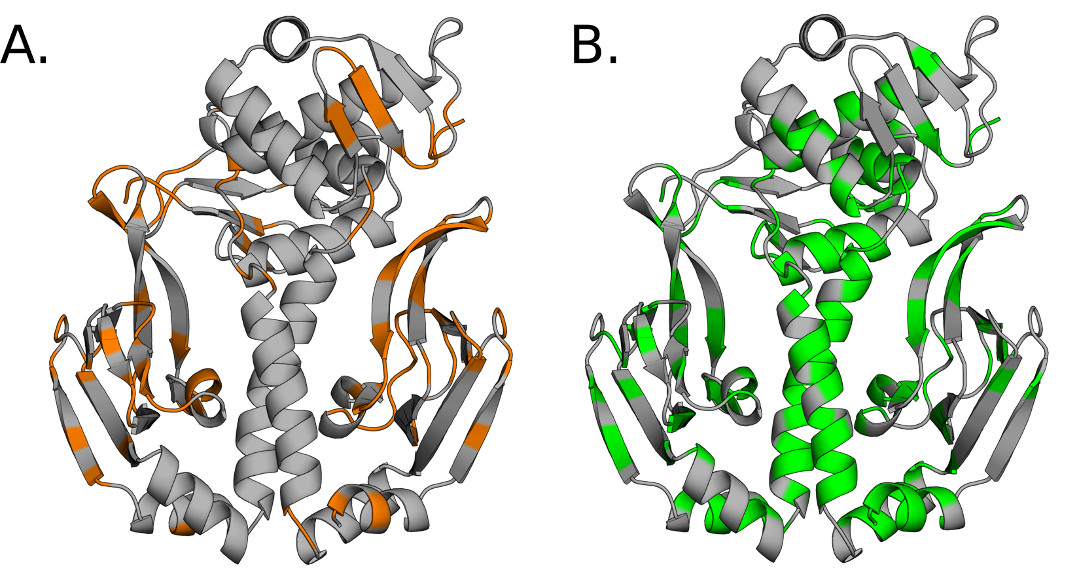
\includegraphics[width=4.5in]{suppfig4-disord-resis-cutoff.png}
    %     \caption[]{Residues with separable dihedrals into disordered regimes using a stricter threshold ($\langle\tau_{ord}\rangle \geq 5\times\langle\tau_{dis}\rangle$) A. Residues with at least one backbone dihedral that is capable of disorder-mediated communication (orange). B. Residues with at least one side-chain dihedral that is capable of disorder-mediated communication (green).}
    %     \label{fig:cards-disord-resis-cutoff}
    % \end{figure} 

    % \begin{figure}[!htb] %Positioning code for figure
    %     \centering
    %     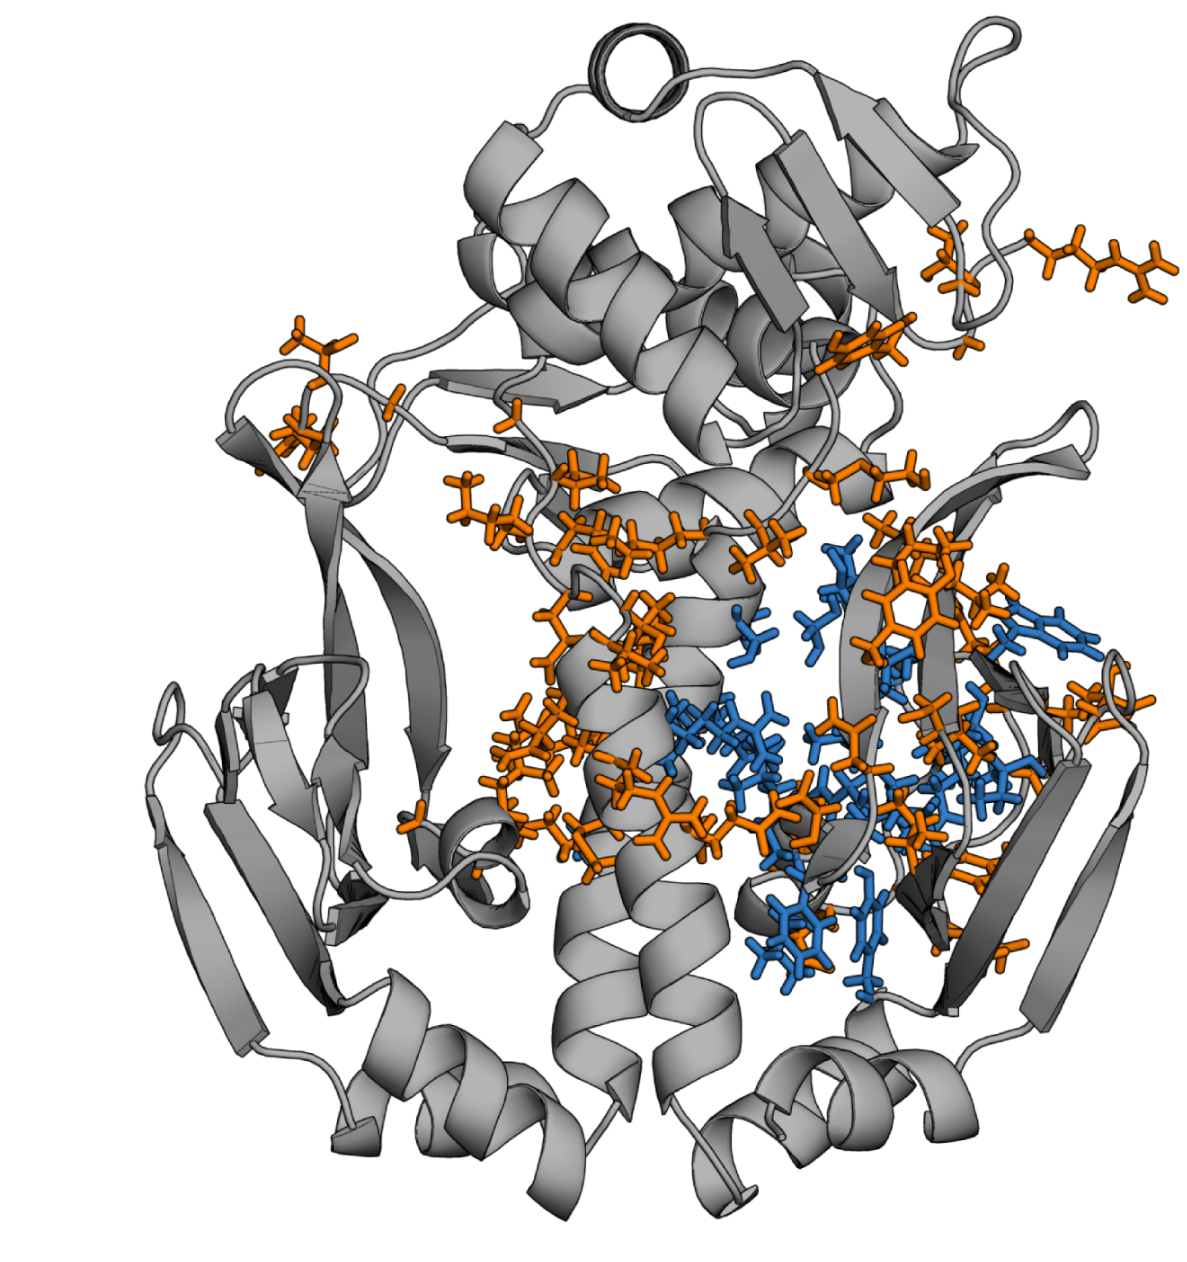
\includegraphics[width=4in]{suppfig5-top5percentresis.png}
    %     \caption[]{The top 5\% of residues (orange sticks) with disorder-mediated communication to the cAMP-binding pocket (blue sticks). Note that having disorder-mediated communication to the CBD does not preclude the possibility of also having structural communication.}
    %     \label{fig:cards-top5percentresis}
    % \end{figure} 

    % \begin{figure}[!htb] %Positioning code for figure
    %     \centering
    %     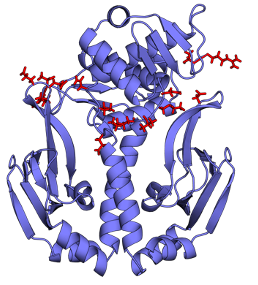
\includegraphics[width=2.5in]{suppfig6-top2percent-hubs.png}
    %     \caption[]{The top 2\% of backbone-side-chain hubs (sticks).}
    %     \label{fig:cards-top2percenthubs}
    % \end{figure} 

    % \begin{figure}[!htb] %Positioning code for figure
    %     \centering
    %     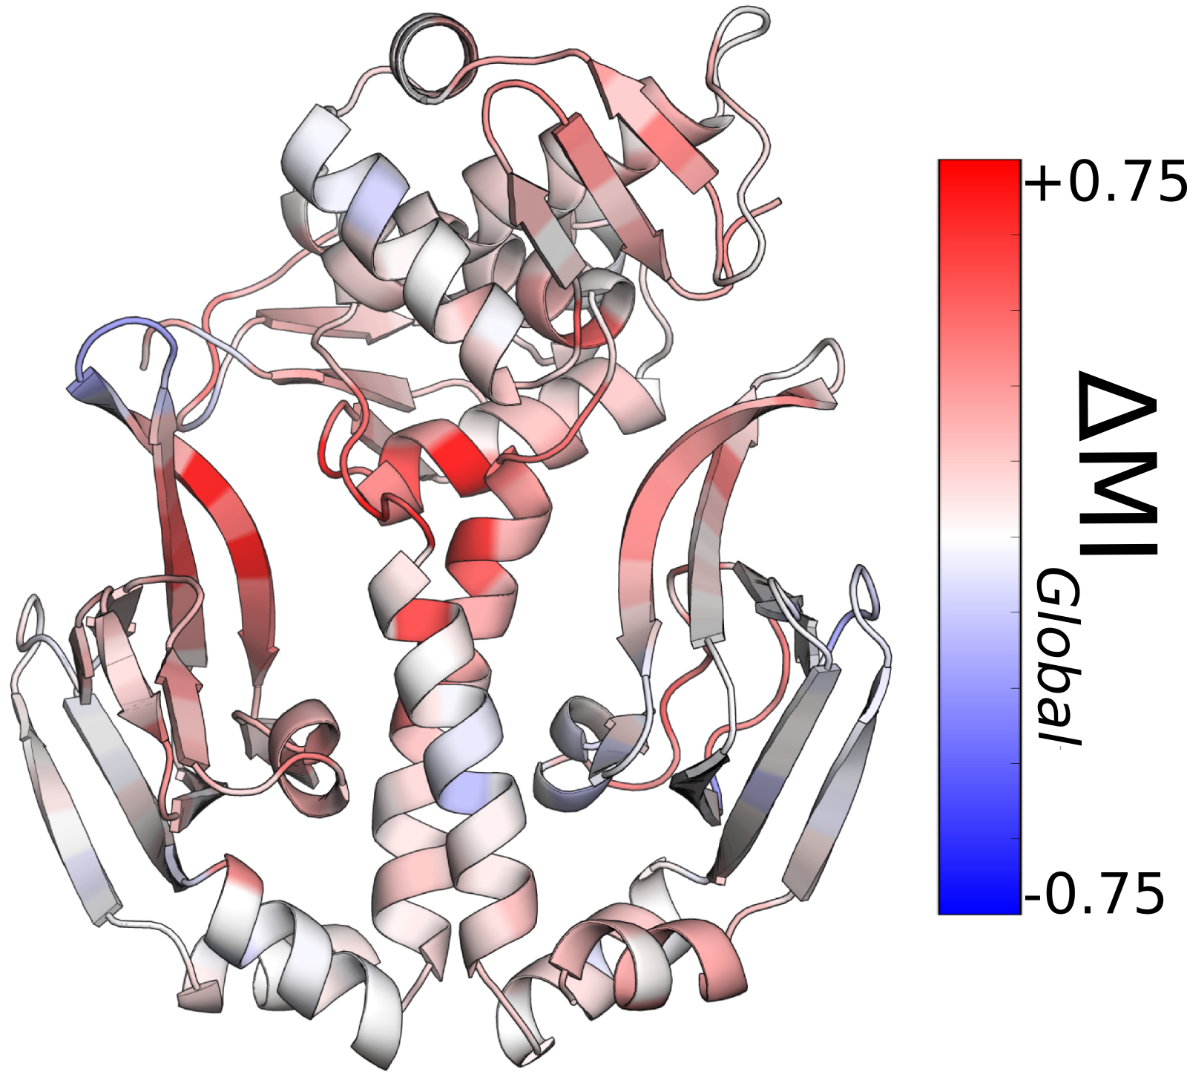
\includegraphics[width=3in]{suppfig7-deltaglobalMI.png}
    %     \caption[]{Change in global communication upon the S62F mutation. The color scale on the right shows the proportional change in global communication relative to the scale in Figure \ref{fig:cap-global-mi-fig} of the main text.}
    %     \label{fig:cap-deltaglobalMI}
    % \end{figure} 

% \bibliography{../References}
% \bibliographystyle{unsrt}

\end{document}